\chapter{总体设计}

\section{设计目标}
LingoBridge 中文自学辅助平台的总体设计目标是构建一个面向中亚留学生的高效、轻量且具备跨国网络容错能力的中文标准拼音听读与多语种词汇对比教学平台。系统在技术实现上通过静态化资源托管与轻量级信令交换机制，有效降低跨国公网长距离传输中的网络抖动负荷，确保拼音发音、大纲跟随及课件展现的流畅性。平台在设计中以拼音听读教学为主线，将复杂的口语跟读评测及实时音视频会议通道列为后续演进方向。同时，系统在开发期支持本地化轻量元数据冷启动，在生产部署后提供向 PostgreSQL 关系型持久化存储的兼容性过渡，以达成低维护开销与高数据一致性的双重目标。

\section{设计原则}
平台在架构设计与技术选型过程中，主要遵循以下四项核心设计原则。

一是职责分离原则。系统在物理与逻辑层面上将静态资源展示、业务逻辑控制以及数据持久化解耦。前端负责页面渲染与交互输入，不涉及物理数据库读写，所有数据变更均通过标准的安全接口上报；后端通过 Repository 仓库层对数据访问进行抽象，将底层的物理读写与上层控制器路由逻辑隔离，提高了系统的模块独立性。

二是跨端一致性与自适应原则。系统前端界面采用响应式自适应布局，以保证在 PC 端及移动端设备上的视觉呈现一致性。系统内置了多语种（中文简体、俄语、哈萨克语）热切换机制，所有的错误提示、导航及教学大纲均由底层的语言上下文模块动态加载。

三是网络容错与计算下推原则。针对跨海公网易产生抖动及连接超时的技术现状，系统在信令交互上引入了自适应指数退避与重连机制。系统在前端推行解析下推策略，利用客户端浏览器内置的 PDF.js 进行课件分页解析与 Canvas 高保真渲染，避免了在服务器端进行高开销解析，降低了跨国数据传输的带宽负担。

四是基于角色的访问控制原则。系统严格落实基于角色的细粒度访问控制机制，无论是对课程大纲的维护、班级成员的管理还是作业数据的导入，均需要在网关层通过 JWT 签名校验。在多租户维度，系统确保不同班级与课程的数据在物理与逻辑层面上实现隔离，防止越权访问。

\section{系统总体架构}
本系统采用经典的前后端分离架构，整体划分为用户交互展现层、业务逻辑控制层、数据存储仓库层以及云端外部服务层。LingoBridge 基于 Vercel 托管与云服务器的部署拓扑架构如图 2.1 所示。

\begin{figure}[H]
\centering
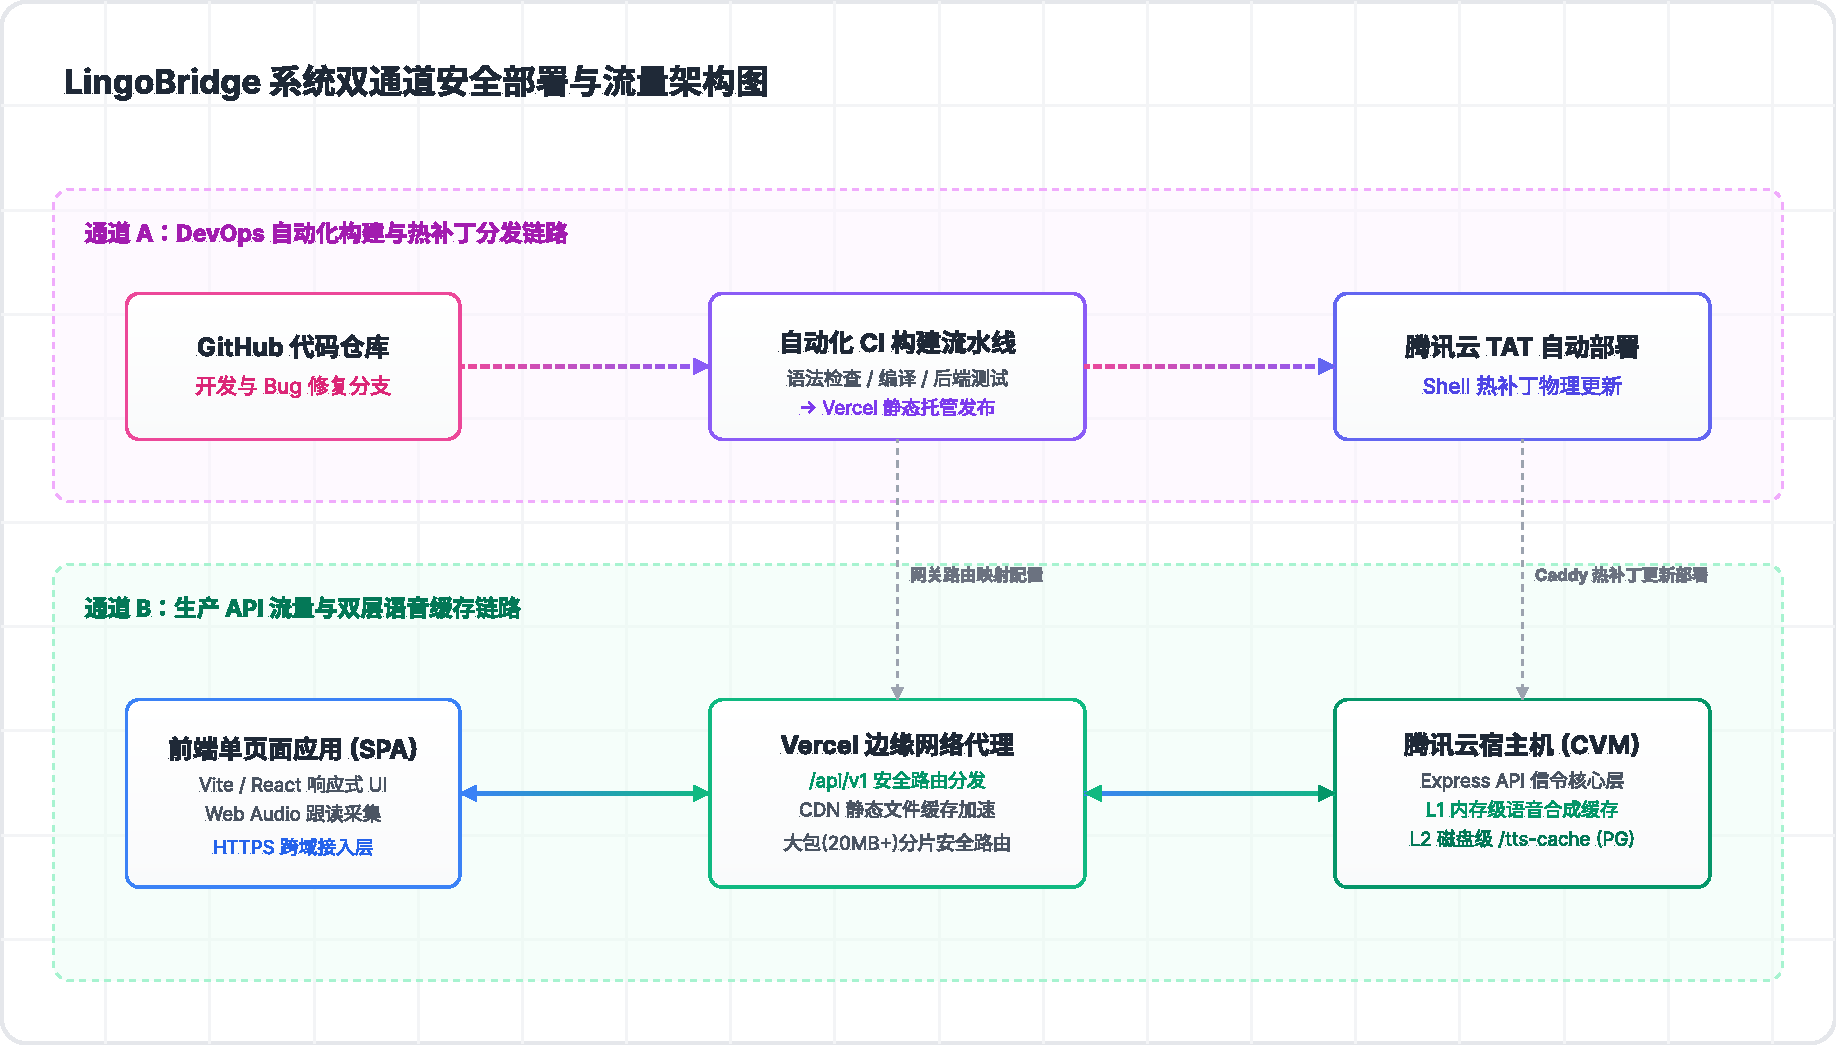
\includegraphics[width=0.65\textwidth]{figures/architecture.pdf}
\caption{LingoBridge 跨国双通道安全部署与流量解耦架构图}
\label{fig:erd_arch}
\end{figure}

根据图 2.1 所示的系统架构，用户交互展现层全部使用 React 19 单页面应用（SPA）构建，静态构建物打包托管于全球 CDN 边缘节点，以降低页面首屏的加载延迟。业务逻辑控制层由部署在服务器上的 Node.js 与 Express.js 4.x 承担，通过标准 HTTPS 协议监听客户端的接口调用与 Presence 状态握手。数据存储仓库层在本地开发模式下支持高内聚的物理 JSON 文件读写，在生产环境中通过切换环境变量，无缝转换为 PostgreSQL 16.0 关系型数据库。云端外部服务层则提供向外部语音合成（TTS）接口以及后续演进的自动语音识别（ASR）评测通道的集成对接。

\section{系统运行环境}
为了确保系统在部署上线及试点运行过程中的稳定性，特制定表 2.1 所示的软硬件及网络运行环境规格要求。在系统实际运维与测试过程中，各项指标均应满足表 2.1 中的规定。

\begin{table}[H]
\centering
\caption{LingoBridge 软硬件与网络运行环境规格表}
\label{tab:run_env}
\begin{tabularx}{\textwidth}{l p{3.2cm} X}
\toprule
\textbf{环境分类} & \textbf{规格/软件配置} & \textbf{具体指标要求与环境功能描述} \\
\midrule
客户端浏览器 & Chrome 100+ / Edge 100+ & 支持标准的 Web Audio API、Canvas 2D 绘图以及 WebSocket 协议，不兼容 IE 等旧版浏览器。 \\
服务端 CPU 与内存 & 腾讯云 CVM (2核 4G) & 主机部署于中国香港节点，主频不低于 2.0 GHz，作为后端信令与数据库的主运行环境。 \\
网络带宽与延迟 & 带宽不低于 6Mbps & 要求跨国往返网络延迟小于 150ms，服务器端支持容器反向代理，对外绑定公网标准 80 与 443 端口。 \\
数据库与中间件 & PostgreSQL 16.0 + Node.js 20 & 采用 PM2 进行 Node.js 进程常驻守护，PostgreSQL 数据库需开启自动事务日志归档与物理隔离。 \\
\bottomrule
\end{tabularx}
\end{table}
